\section{Directory structure}
The framework is written in Go and it contains few custom Go
packages\cite{Packages-go} that can be further extended, that is
\begin{itemize}
\item \verb|main| --- package that every go application needs to have in order
  to be executable, from this package binary file will be
  created\cite{Packages-go},
\item \verb|common| --- contains common utilities that are used across whole
  framework,
\item \verb|config| --- contains package that is obliged to manage yaml based
  config files dependent on environmental variable,
\item \verb|middleware| --- contains middlewares, small plugins that modify
  requests and responses.
\end{itemize}

In \verb|main| package few very important files were created
\begin{itemize}
\item \verb|main.go| --- every go application has a \verb|main| function which
  is a so called entry point,
\item \verb|routes.go| --- contains routes definitions as described in
  (\ref{sec:path-of-the-request}),
\item \verb|router.go| --- contains function for setting up routes defined in
  \verb|routes.go| file, default middlewares could be changed there
\end{itemize}

\section{Building}

\subsection{Prerequisities}
In order to build the project you need to have installed the following
\begin{itemize}
\item Go\footnote{\url{https://golang.org/dl}},
\item Git\footnote{\label{git-src}\url{https://git-scm.com}} (optionally).
\end{itemize}
Then you need to set up the two environmental variables
\begin{itemize}
\item GOPATH\cite[The GOPATH environment variable]{Packages-go} --- which
  points to your workspace directory,
\item PATH --- which should be extended by one one additional path
  \verb|$GOPATH/bin|
\end{itemize}

\subsection{Getting source code}
The application is stored on GitHub. In order to build it, one should fetch it
at first. There are two approaches to this problem.

First, head over to website
\begin{verbatim}
github.com/dolohow/go-http-framework
\end{verbatim}
Search for the button ``Download ZIP'' and click it. Download process will
begin, after it is finished unpack it with any program of your
choice\cprotect\footnote{For UNIX users issue a command
\verb|unzip master.zip|.}.

Second, requires git\footnotemark[\getrefnumber{git-src}] and comes down to one
command
\begin{verbatim}
go get github.com/dolohow/go-http-framework
\end{verbatim}
which will clone the whole repository with code to your current working
directory\cprotect\footnote{For UNIX users type \verb|pwd| to find out.}.

\subsection{Compiling \& Running}
To compile the project navigate to
\begin{verbatim}
$GOPATH/src/github.com/dolohow-go-http-framework
\end{verbatim}
and issue a command \verb|go install|. It will compile and put the binary file
into your \verb|$GOPATH/bin|. If you set up your PATH properly you should now
be able to invoke the program just by typing its name in console.

In addition you can specify the port that the program will be listening on by
\verb|-port| switch\cprotect\footnote{For more information run program with
\verb|--help| switch.}.

\section{Principles of operation}

\subsection{Path of the request}
\label{sec:path-of-the-request}
Server by default listens on port 5000. For every request the new
Goroutine\cite{Goroutines-go} is being created. It is similar to
thread\cite{Programming-in-go}, but basically it comes down to being a thread
under the thread. Therefore every new request is handled separately and does
not block the new requests. Such behaviour is provided by
\textit{http}\cite{HTTP-go} package by default.

How can the application differentiate between one request or another? We need
to have some sort of routing mechanism. As stated in~\ref{sec:resources} every
resource is identified by URI, therefore for every URI new handler needs to be
created.

For that, special type \textit{Route} was created in order to link handlers
with URIs (Path) as well as HTTP method (\ref{uniform-interface}). In addition
it can pass the request data by specified list of middlewares.

\begin{verbatim}
type Route struct {
        Method      string
        Path        string
        Middlewares []middleware.Middleware
        HandlerFunc http.HandlerFunc
}
\end{verbatim}

\begin{figure}[!htbp]
\begin{verbatim}
Route{
        "POST",
        "/register",
        Middlewares{
                middleware.AuthWithJwt,
                middleware.BodyParser(user.User{}),
        },
        user.RegisterHandler,
}
\end{verbatim}
\renewcommand\figurename{Code}
\caption{Example route}
\label{src:example-route}
\end{figure}

When new request arrives the requested resource is searched linearly in array
consisting all \textit{Route} definitions. When it is not found then 404 Not
Found status error code is sent. Then it is client job to handle that properly.
When it is found, then the request object is piped to first default middleware.
Those are mandatory, like setting proper response headers, next through
middlewares specified in Route object. After last middleware being finished the
handler is going to be executed. In handler one can set status code, body of a
response like JSON object, fetch data from database and so on.

\subsection{Building custom middleware}
Function that can be treated as a middleware must accept
\verb|http.Handler|\cite{Go-Phrasebook} usually named \verb|next| as a
parameter and return \verb|http.Handler| as well. To create a
\verb|http.Handler| use \verb|http.HandlerFunc| which is an
adapter\cite{HTTP-go} defined as:
\begin{verbatim}
type HandlerFunc func(ResponseWriter, *Request)
\end{verbatim}

Now you can see that you also need to create an ordinary function with\\
\verb|ResponseWriter| and \verb|*Request| parameters where you can modify those
and after you finished you should call \verb|ServeHTTP| method on
\verb|http.Handler| in order to pass execution context to the next middleware
or a handler. If you will not do this the response and request will never reach
the handler and the client will never see a response. This function is usually
defined inside function middleware as anonymous function, but it does not have
to.

\begin{figure}[!htbp]
\begin{verbatim}
func SetJSONHeader(next http.Handler) http.Handler {
        handler := func(w http.ResponseWriter, r *http.Request) {
                w.Header().Set("Content-Type",
                        "application/json;charset=utf-8")
                        next.ServeHTTP(w, r)
        }
        return http.HandlerFunc(handler)
}
\end{verbatim}
\renewcommand\figurename{Code}
\caption{Example middleware that sets response headers}
\label{src:example-middleware}
\end{figure}

\subsection{Creating handler}
Handler is the last function that will be executed in execution chain
(\ref{fig:middleware}) after all middlewares completed. The word ``Handler'' is
suffixed to a function name in order differentiate between other functions.

It accepts two parameters, first \verb|http.ResponseWriter| and
\verb|*http.Request|. Request object contains \verb|Method|, \verb|URL| of
resource, \verb|Body|. Those are the most important and often used. When you
are finished with creating response, write it to a \verb|ResponseWriter| using
\verb|fmt.Fprintf| or anything else that can write to \verb|io.Writer|
interface.

\subsection{Authentication mechanism}
As stated in (\ref{sec:stateless}) every request needs to carry authentication
data. This kind of data is usually called token. It can be randomly generated
and then saved in database. Then request token is compared with the one saved
in database. In case they are different the user is not authenticated or
malformed token. Otherwise we assume the request was authenticated.

But there is a better approach. Instead of storing every token in database
(which is harder to test, it requires mocking database or having a running
instance). We can sign the string and then verify the signature of incoming
request token.

\subsubsection{Principle of operation}
Let us say the client wants to register on our website and the backend is
RESTful. First he needs to make a POST request to defined resource (i.e.
\verb|/register|) with required data such as an email and a password. We
validate those in handler and if the data is correct token will be sent to the
user in response.

The client saves the token and attaches it to every request so we can be sure
that he is the person who claims to be.

\clearpage
\begin{figure}[!htbp]
\centering
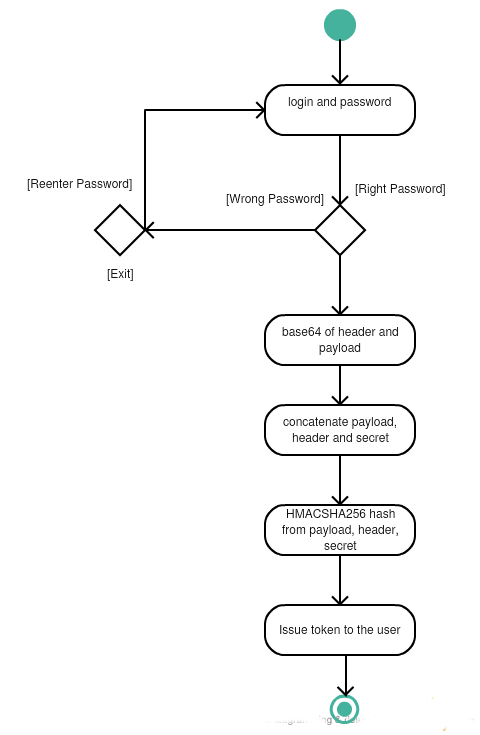
\includegraphics[scale=0.6]{auth}
\label{fig:auth}
\caption{Activity diagram of token creation}
\end{figure}

\subsubsection{Token demystified}
How the token looks like? It is a string contains three parts separated by
``.'' character\cite{JWT-introduction}. Those parts represents
\begin{itemize}
\item Header,
\item Payload,
\item Signature
\end{itemize}

Header, typically contains type of token and hashing algorithm. Then it is
encoded by Base64Url algorithm.
\begin{figure}[!htbp]
\begin{verbatim}
{
    "alg": "HS256",
    "typ": "JWT"
}
\end{verbatim}
\caption{Typical header of JWT token}
\label{src:typical-header}
\end{figure}

Payload, contains so called claims. Those contains data about entity (usually
the user) and additional metadata. There are three types of claims
\begin{itemize}
\item Registered names, those are reserved and defined by RFC standard. They
  can contain information like expiration date of the token\cite{JWT-rfc},
\item Public names, they can be defined by the user, like email address, set of
  privileges, but the creator is responsible for creating namespace to avoid
  collisions,
\item Private names, created to share information that both parties agree on
  using them.
\end{itemize}
Then encode that with Base64Url algorithm.

To create signature, take the encoded header, encoded payload. Concatenate them
with ``.'' and use secret\footnote{It is randomly generated string only known
to you} to sign that with algorithm of your choice. Then it is used to verify
the authenticity of the token and validate data (header and payload).

\begin{figure}[!htbp]
\begin{verbatim}
HMACSHA256(
    base64UrlEncode(header) + "." +
    base64UrlEncode(payload),
    secret)
\end{verbatim}
\renewcommand\figurename{Code}
\caption{Pseudocode that generates signature from header and payload}
\label{src:signature}
\end{figure}

